
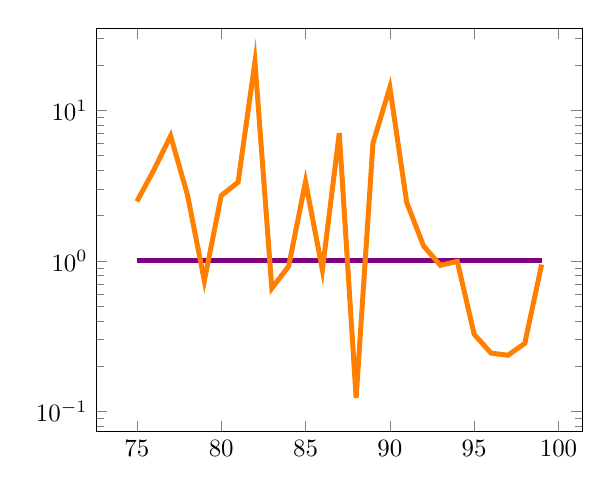
\begin{tikzpicture}[scale=0.9]
\begin{semilogyaxis}
\addplot[color=violet,line width=2pt] coordinates {(75,1.0)(76,1.0)(77,1.0)(78,1.0)(79,1.0)(80,1.0)(81,1.0)(82,1.0)(83,1.0)(84,1.0)(85,1.0)(86,1.0)(87,1.0)(88,1.0)(89,1.0)(90,1.0)(91,1.0)(92,1.0)(93,1.0)(94,1.0)(95,1.0)(96,1.0)(97,1.0)(98,1.0)(99,1.0)};
\addplot[color=orange,line width=2pt] coordinates {(75,2.482883076277859)(76,4.001522951915039)(77,6.752494384205922)(78,2.7419226045531278)(79,0.7383427366115699)(80,2.711820113405769)(81,3.3279190668265177)(82,20.99839174074961)(83,0.6574413545777595)(84,0.9211164506471073)(85,3.3570247725163167)(86,0.8709883908235574)(87,7.052652185738737)(88,0.12280655881843916)(89,6.063058021120462)(90,14.202200595206836)(91,2.4421751760785364)(92,1.2552994441240872)(93,0.9340598964247149)(94,0.9927686249037149)(95,0.32534489808406203)(96,0.24408954731109256)(97,0.23626034630323256)(98,0.28301757862289034)(99,0.9452340885105958)};

\end{semilogyaxis}
\end{tikzpicture}
